\documentclass{article}

\usepackage[parfill]{parskip}
\usepackage{graphicx}
\usepackage[utf8]{inputenc} % For åäö

\title{Suggested solution}
\author{Mattias Fält, Lucas Jimbergsson,\\Erik Nossborn, Iulia Stoica}

\begin{document}
\maketitle

\section{Regulator structure}\label{regstruc}
We are planning to use different regulator structures for the different parts of the execution. The idea is that we will use a simple PID controller to move the beam to the pick-up position and then a LQG regulator for the other parts.
\subsection{Step 1, Beam control}
We will use a simple PID controller for the position of the beam in this part. A gradually increasing reference will be given for the beam until indication is given that the beam is in the pick-up position. The reference will then stay constant until the next controller is started. The controller for this part is governed by the BeamRegul class.
\subsection{Step 2, Ball balancing}\label{step2}
This part will be regulated by a time-invariant LQG regulator. The model will thus be linearized around the desired position for the weighing. If this proves to be not robust enough (for all weights of the balls), we might introduce the ball weight as a parameter in the model, which can be estimated by the Kalman-filter. We might switch to a cascaded PID controller if this method is too hard to implement or is taking too much time.
\subsection{Step 3, Ball delivery}
We will have the same structure for all controllers in this part but they will have different reference values. The idea for all of them is to first find a nominal solution to the nonlinear equations and then control the system using time-varying LQG regulators. It might be beneficial to have an intermediate regulator that move the system to a state different from the weighing state, before we exectute these controllers, to get a better initial state for the optimization method described below.
\subsubsection{Finding a solution}
We have several ideas on how to solve this part. We can either use JModelical to find an optimal trajectory similar to what is done in Nonlinear Control Lab 3. If this requires too much time, we might also use a numerical optimization approach in MATLAB, as outlined in for example \cite{NR} chapter 21.1.1. Lastly, if these methods fail or provide unsatisfactory solution, we could make a simple ansatz and find an analytical solution.
\subsubsection{Calculating regulator}
The method above would generate a trajectory that satisfies the specific goal for the current ball. We can then, using MATLAB, solve the differential Riccatti equation for the linearized time-varying system using some simple numerical solver. This would generate a feedback and estimation matrix for each timestep which can be saved to disk.
\subsubsection{Executing regulator}
Each regulator can read its respective feedback and estimation values for each time-step at initiation and will then simply apply them in real time.


\section{Transition between controllers}
When going from one controller to another, the control signal may very well make a jump from one value to another. The bumps introduced may be problematic if they are considerable and not dealt with. As compared to the newer \emph{ball and beam} process used in Lab 1 however, our older process has an extra integrator (torque instead of angular velocity as input signal) which gives an even stronger lowpass behavior. This will indeed smooth the bumps but we will have to investigate whether, and to what extent, we have to deal with them.

One idea we have for dealing with bumps, is to initially run the control signal through a lowpass filter after a switch of controller. In the initial time frame when lowpass filtering is active however, the controller will be slow, so the filter has to be deactivated before we allow the reference signal to change.

\section{UML}

An overview of the classes is showb in figure fig fig. 
The responsabilities of each class are as follows:
\begin{itemize}
\item Main: the constructor creates an instance of the first controller to be run and it also creates and starts an instance of its internal thread called MainThread. This thread is the one performing the calculations of the control signal with the help of methods of the current controller.
\item Regul: is an abstract class which all the controllers inherit from. It contains a thread whose task is to check if the work of the currently running controller is finished and it also checks if the program should switch to a different controller. It has an internal monitor called ParamMonitor which communicates with the Gui thread. The RefBeamMonitor is valid only for the controller of the beam only.
\item Measurement and OutSignal are help classes, the first containing measurement signals and the latter containing the outputs
\end{itemize}

\begin{figure}[htbp]
  \centering
  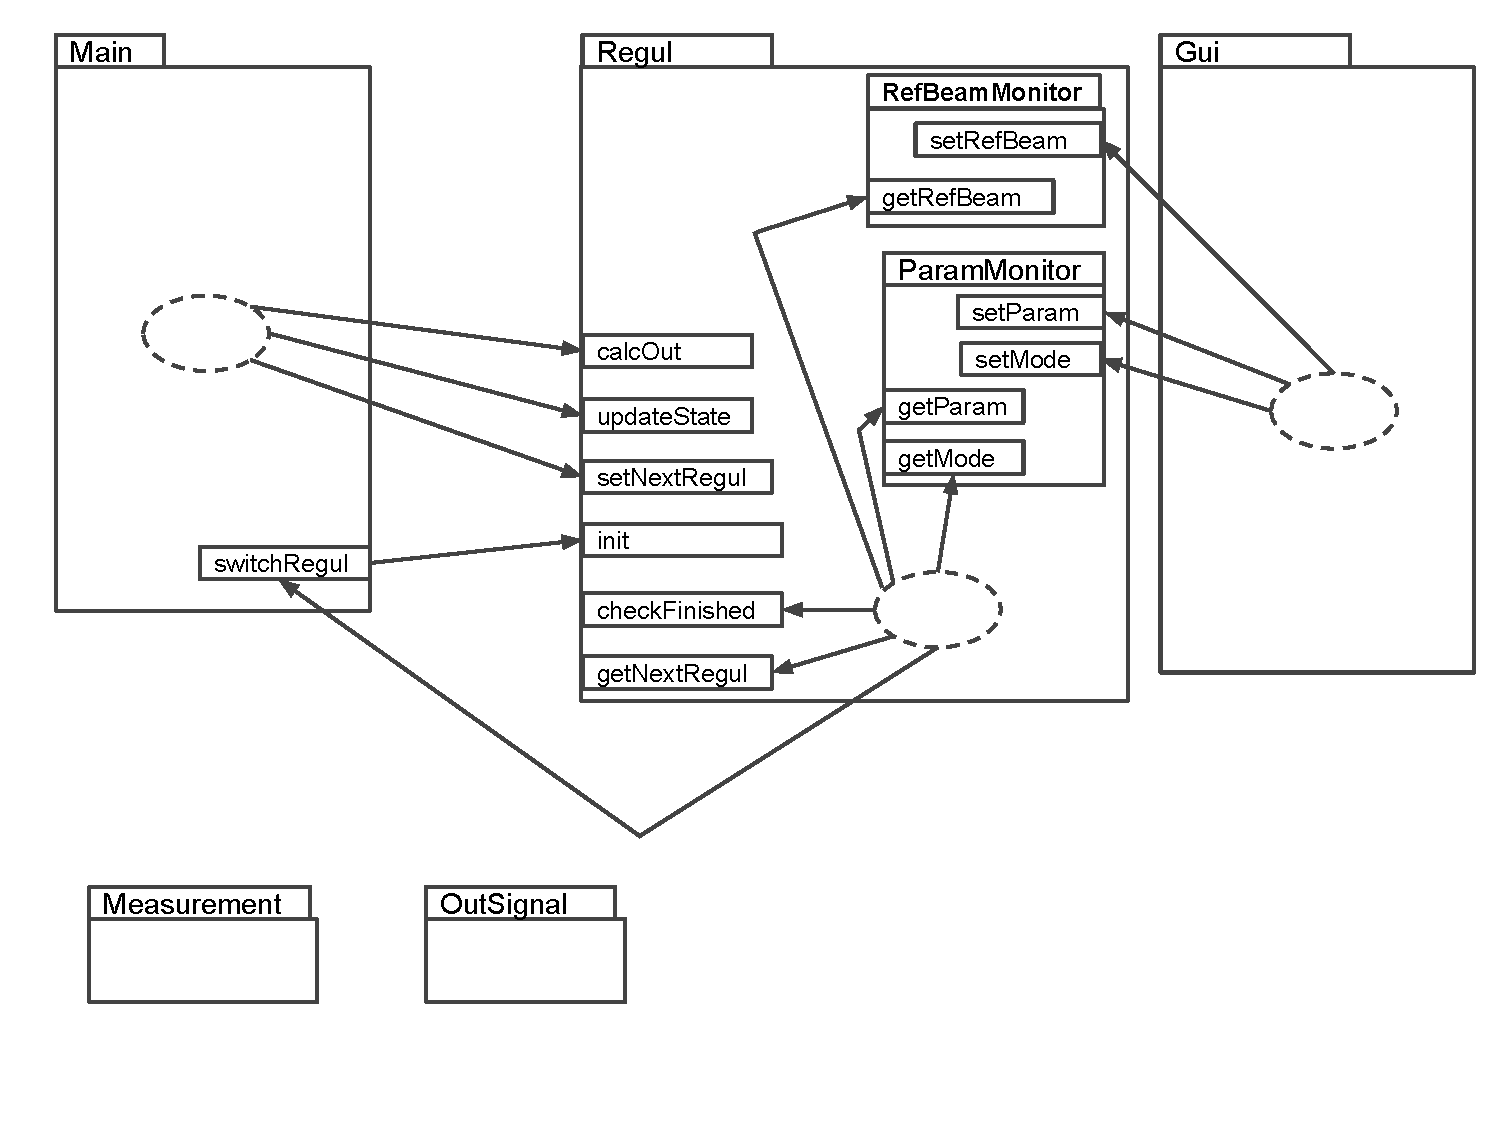
\includegraphics[width=\textwidth]{UML}
  \caption{UML diagram}\label{fig:UML}
\end{figure}

\section{Operator communication}
\subsection{Plotters}
We will have the following plotters:
\begin{itemize}
\item Beam position (reference, measurement and Kalman filter estimate)
\item Ball position (reference, measurement and Kalman filter estimate)
\item Control signal
\end{itemize}

\subsection{Modes}
We intend to implement three different modes; Beam control, Ball balancing and finally the entire sequence control scheme described in section \ref{regstruc} (beam control, ball balancing, ball delivery).
\subsubsection{Beam control mode}
In this mode only the beam will be controlled by a PID controller. The user should be able to tune the PID parameters as well as altering the reference value online.

\subsubsection{Ball balancing mode}
As discussed in section \ref{step2}, either LQG or cascaded PID will be used when balancing the ball for measuring its weight, and the ball balancing mode will use the same controller.

If cascaded PID controllers will be used, the user will be able to tune PID parameters as well as altering the reference value for the ball. If LQG will be used however, controller parameters (weighting matrices and noise intensities) will not be as straight-forward to change online (the Riccati equations need to be resolved by some Java package or Java-\textsc{Matlab} communication). Also a reference value change would affect the linearization point, and a relinearization would be appropriate although for the same reason not very straight-forward. Therefore, with an LQG setup the controller parameters as well as reference value will only be able to change online if time permits.

\subsubsection{Sequence control mode}
In the sequence control mode, we want to test the performance of the full sequence when adjusting parameters. Therefore, a change of parameters in this mode should only affect the following iteration, and not the current one.

As for the previous mode, online Riccati resolving and relinearization could be difficult to achieve. Nevertheless the user should be able to tune PID parameters as well as change the position interval for the beam when searching for the correct position to pickup a ball. If time permits, also some of the following could be allowed for an online change:
\begin{itemize}
\item LQG weighting matrices for ball balancing
\item Desired ball position when estimating its weight
\item LQG weighting matrices for ball delivery
\item Desired final state for ball delivery
\item LQG noise intensities (same for balancing and delivery)
\end{itemize}

\section{Timetable}
\subsection{Workflow}
The following tasks are equivalent to those described in section \ref{regstruc}:
\begin{enumerate}
	\item Get beam into position to receive ball
	\item Weigh ball
	\item Throw ball
\end{enumerate}
\subsection{Schedule}
\begin{tabular}[h]{|l|p{10cm}|}
\hline
Week & Things to do \\ \hline
45 (3-9 Nov) & *Sketch a preliminary solution of the problem and create timetable \\
 & *Code for regulation of beam (part 1) and ball \& beam (part 2) will be ready for testing individually on the real process  \\
 & *Have a precise list with all steps required for creating an LQG regulator, ie theoretical model, Riccati equation, estimation of other parameters that are needed (all the theory, basically). Write all these in the LaTeX document to make report writing easier later \\
 & *Structure for the whole program will hopefully be ready (with potential suggestions from Karl-Erik), ie which classes and threads we will have and how they interact \\
\hline
46 (10-16 Nov) & *Hopefully we can now start testing on the real process, test with the regulator for beam only (part 1) and the one for beam \& ball (part 2), as well as estimation of parameters in the model (needed for stage 2) \\
 & *Parallel work: Two people can work on part 1 and two on part 2 \\
 & *GUI for the program \\
\hline
47 (17-23 Nov) & *Continued work on part 1 and 2 \\
 & *Start testing part 3 \\
\hline
48 (24-30 Nov) & *Refine part 3, Kalman filter, improvements of stuff \\
\hline
49 (1-7 Dec) & *Refine part 3 \\
\hline
50 (8-14 Dec) & *12 Dec hand in report, prepare presentation \\
\hline
51 (15-16 Dec) & *Demonstration and presentation 16:th of Decemeber at 15:15 and 17:15 \\
\hline

\end{tabular}

\newpage
\begin{thebibliography}{9}
\bibitem{NR}
  Thomas Bewley,
  \emph{Numerical Renaissance: simulation, optimization, \& control}.
  Renaissance Press,
  http://numerical-renaissance.com/NR.pdf

\end{thebibliography}

\end{document}
